%% American Dream Stuff

The American Dream is long-hailed as one of the most prosperous and ambitious ideals reaching wide-scale popularity. Within the United States, the ideology behind the `American Dream' provides a positive notion towards the attainability of wealth and financial freedom. 
This claim also argues that mobility of economic quintiles can, and will be achieved by any motivated American who envisions establishing an economic foundation. But, is this a notion of reality? 
The phrase `The American Dream' was first introduced by historian and writer James Truslow Adams in 1931. Adams coined the phrase in his book The Epic of America which emphasized the enterprising concept of financial achievement. 
According to Adams in The Epic of America, he describes the American Dream as, `that dream of a land in which life should be better and richer and fuller for everyone, with opportunity for each according to ability or achievement' \parencite{adams2017}.
%% if want to use that graph from chetty
\begin{figure}
    \caption{Source: \cite{opportunityinsights}}
    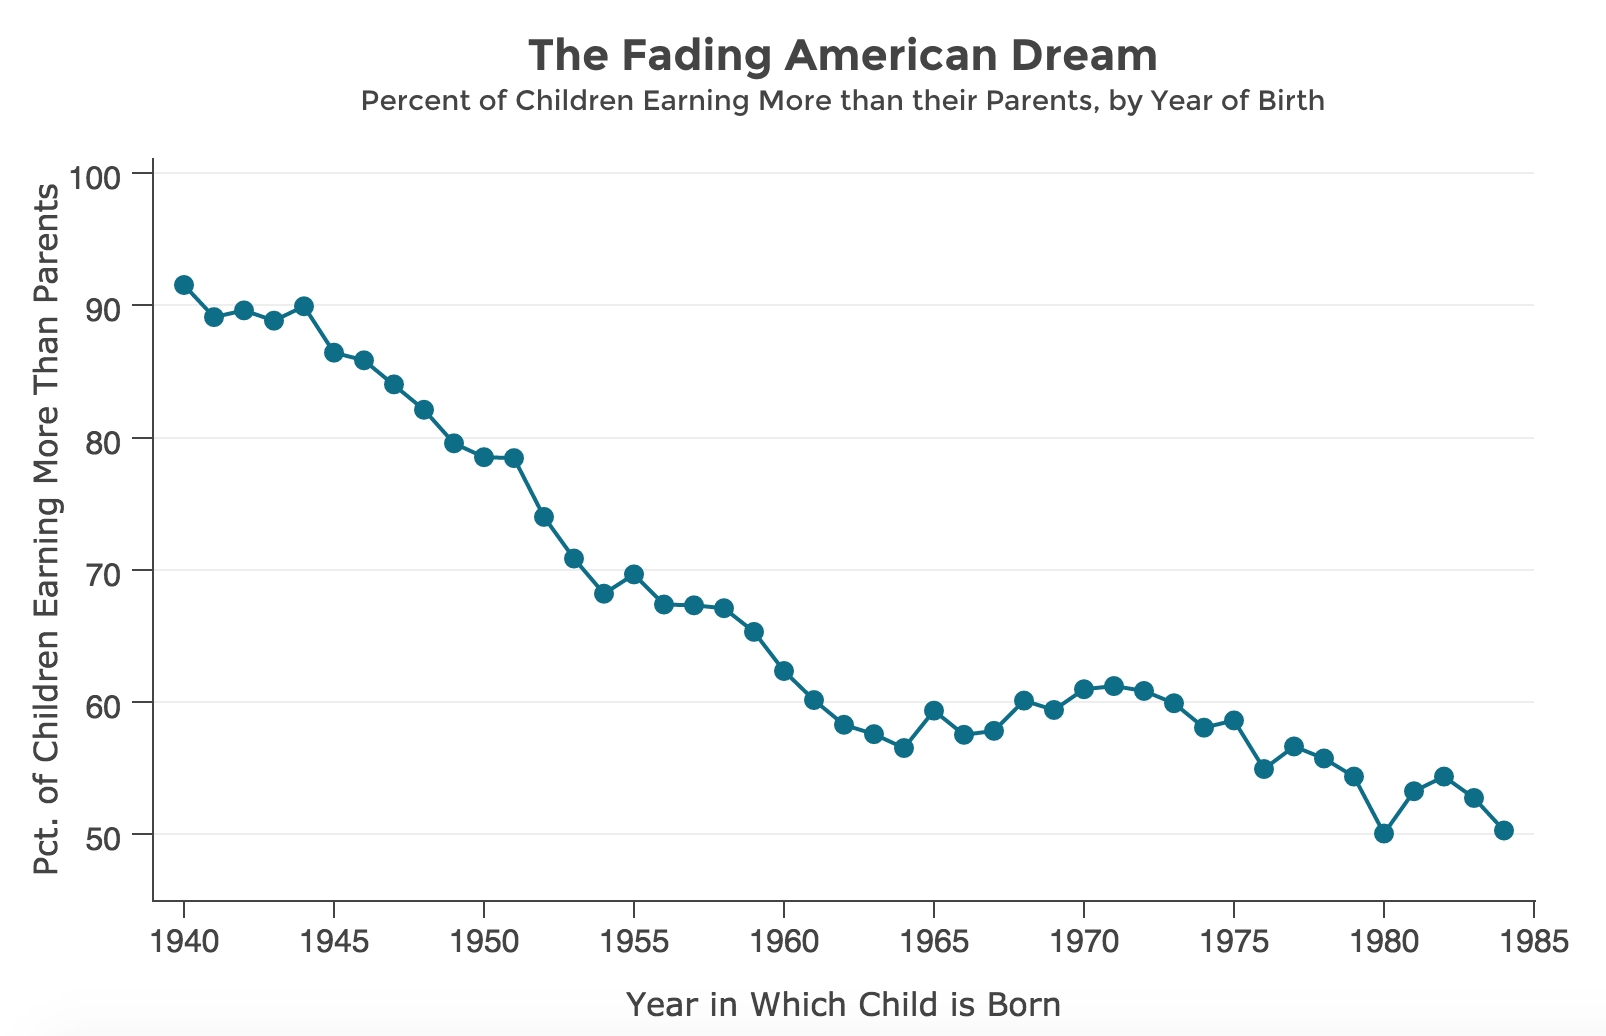
\includegraphics[width=17cm]{chetty_economic_mobility.png}
    \label{fig1}
\end{figure}





%%%%%%%%%%%%%%%%%% rest of overview

Opportunity Insights is a non-profit and partisan organization operating out of Harvard University in Massachusetts. They focus on research using large datasets to locate economic inequity. 
The team has experts in a variety of fields, using the collective disciplines to formulate solutions in battling inequality and poverty \parencite{opportunityinsights}.
Opportunity Insights is led by Director Dr. Raj Chetty, Professor of Economics at Harvard. 
As part of a broader research initiative to examine the impacts `of  tax  expenditures  on  the  budget  deficit  and  economic  activity', Chetty and his colleagues published the 2014 paper `Where is the Land of Opportunity? The Geography of Intergenerational Mobility in the United States', inspecting economic mobility of the fifty largest cities in the United States, and exploring the classic idea of the `American Dream' \parencite{opportunityinsights, chetty2014}.
Economic Mobility in this case was defined as moving from the bottom fifth income group to the top fifth group. 
They found that mobility was linked with racial and income segregation, income inequality, school quality, access to social capital, and family stability \parencite{chetty2014}.
Areas with high economic mobility were also found to have less segregation and income inequality, while having better schools, stable families, and a larger amount of social capital\parencite{chetty2014}.
Charlotte, North Carolina (NC) was included in this report, and ranked last in terms of economic mobility (Chetty et al., 2014, p. 1). Mecklenburg County was found to be 99 out of 100 counties in terms of economic mobility \parencite{opportunityinsights}. This shocked those who saw Charlotte as a growing economic hub in the South-East, but not the residents of Charlotte struggling with this economic disparity. 

In response, the city of Charlotte formed the Opportunity Task Force to address barriers of economic mobility and find solutions \parencite[][]{LOO}. The Task Force met with over 50 experts to understand the issue of intergenerational poverty, and thousands of local residents that experience this inequality first-hand \parencite[][p. ii]{LOO}. 
After 18 months of research, the Task Force published it's recommendations and formed Leading On Opportunity \parencite[][]{LOO}, a board to oversee the implementation of the recommendations in Mecklenburg County in March 2017 \parencite[][p. ii]{LOO}. 
The Task Force identified three key determinants of economic mobility and two cross-cutting factors that have an effect on all three determinants. 
Family Stability, Early Care and Education, and College and Career Readiness were the three major components to a child's ability to climb the economic ladder. Segregation (both racial and income) and Social Capital were the cross-cutting factors that can deeply affect a child's growth. 
Charlotte has a history of racial and economic segregation. 
The poor and minority neighborhoods form a `crescent' shape, while the white and rich neighborhoods are clustered in a `wedge' within the crescent \parencite[][p. iii]{LOO}. 
The home of students determines the school they go to, and in turn, the area around a school can determine the funding. It is because of this that segregation is a key issue that cannot be ignored in any three of the determinants.
\\

Likewise, social capital is associated with higher income students. Those from low-income areas may not have the resources to succeed in school that other students do \parencite[][p. viii]{LOO}. 
Safe places to study, knowledgeable and helpful mentors, and broad social networks are often not as readily available to low-socioeconomic students \parencite[][p. viii]{LOO}. 
A community that is invested in its young people and a bright future for the city is essential in increasing social capital for students \parencite[][p. iv]{LOO}. 
The Opportunity Task Force not only identified these determinants and factors, but also devised changes to be made structurally in 
Charlotte to mitigate economic barriers \parencite[][p. ii]{LOO}.
This plan included 91 recommendations, each with several implementation tactics \parencite[][p. ii]{LOO}.





\begin{figure}
    \caption{Median Household Income of Zip Code Each School Resides In}
    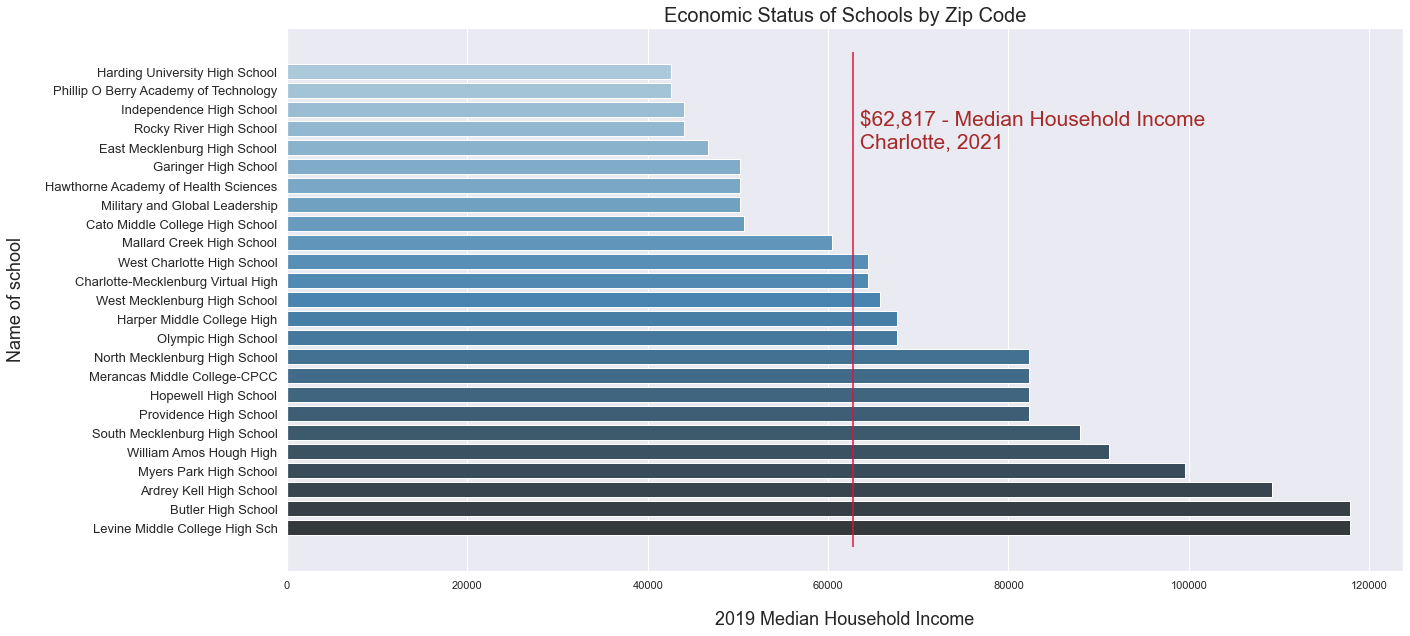
\includegraphics[width=17cm, height=10cm]{school_income.png}
    \label{fig2}
\end{figure}
Our team is focusing on Career and College Readiness in Charlotte-Mecklenburg Schools (CMS), specifically at the high school level. 

Career and College Readiness is a broad term, but generally speaks to a student's ability to enroll and succeed in college, as well as their ability to enter the workforce successfully. Charlotte-Mecklenburg Schools, much like the city itself, is a school district segregated by race and wealth. See Figure \ref{fig2} for median income by school zip code.


The demographics district wide do not represent the demographics at each school. 

\blockquote[Task Force, 2017 p. 14][]{\dots with about 39 percent, black, 29 percent white, 23 percent Latino and 6 percent Asian.\(_{9}\) A third of the 168 schools in the system are segregated by poverty, half are segregated by race and a fifth are hyper-segregated, meaning that 90 percent of their students are from a particular race.\(_{10}\) 
Over half of all African American students attend schools that are 90 percent non-white. 
The majority of white students attend majority-white schools in our high-growth southern and northern suburbs where most of our new schools have been built in recent years, as well as in more affluent close-in neighborhoods such as Myers Park and Eastover.}

With growing economic disparity, further hardships for Charlotte children should be mitigated to increase their socio-economic potential, whether that is perceived or real because of structural barriers. According to a Georgetown University study by Carnevale et al., “two of every three new jobs now require some level of postsecondary education—training credentials, an associate degree, a four-year degree, or higher” \parencite[as cited in][p. 26]{LOO}.

The actual factors that are required to guarantee a student's success is unknown \parencite[][p. 27]{LOO}. 
This is why every avenue of assistance to increase a student's ability to succeed should be explored. 
College can lead to future success, but technical jobs should not be written off as the requirements for those jobs evolve \parencite[][p. 27]{LOO}. 
College Readiness can be increased by more exposure to college-level studies and rigorous courses, arming students with knowledge and information ahead of their future life choices, and increasing their access to social capital. 
This can be accomplished through dual enrollment courses, such as the Career and College Promise Program, giving students access to college courses while in high school through Central Piedmont Community College (CPCC).
Guidance counselors can provide social capital to students with little or none  through their knowledge of college or career resources the students may not otherwise come into contact with \parencite{tang2019high}.
Career Readiness can involve being prepared for college, but equipping students with the knowledge and skills to succeed in the workforce out of high school is essential in preparing students for careers. 
Career and Technical Education (CTE) courses can provide students with the ability to attain relevant credentials, increasing their ability to find gainful employment immediately following graduation. Internships in the community is a way to build social capital for students while still in high school, building their network of employer contacts and recognition in the community. Also, internships can lay the foundation for full-time employment at the same company. 
Paid internships can provide supplemental means to students that would otherwise need to work at a job, freeing their time away from financial obligations by simultaneously compensating students and increasing their career-related experiences. 
By broadening the access of opportunities to more students, especially to low-socioeconomic students, Charlotte-Mecklenburg Schools can further their part in increasing the socio-economic growth of children from Mecklenburg County. 
As said best in Sprint 1, `In the end, it will not be just the high schools that need to prepare the future workforce, but it will take a partnership of primary, secondary, postsecondary, and community organizations to effectively leap the hurdle of economic mobility' \parencite[][p. 2]{sprint1}.